\chapter{Esperimenti e risultati}
\label{chap:esperimenti}

La maggior parte degli attuali studi di previsione della personalità si sono concentrati sull'applicazione di tecniche generali di apprendimento automatico per predire i tratti di personalità Big Five.
In particolare verranno utilizzate diverse strutture di rete, combinando differenti domini.

\section{Spazi di rappresentazione}
\label{sec:approcci}
Per affrontare questo problema di \emph{Text Mining}, gli esperimenti si concentrano su due principali metodi per l'estrazione delle caratteristiche del testo:
\begin{itemize}
	\item Un approccio supervisionato, in cui viene utilizzato come strumento di generazione di feature un vettore \emph{bag-of-words} o brevemente BoW, una rappresentazione di testo che descrive la presenza delle parole all'interno di un documento, in questo caso nel dizionario delle occorrenze \cite{wallach2006topic}.
	\item Un approccio non supervisionato, in cui viene costruito un embedding, tramite l'algoritmo \texttt{word2vec} di Tomas Mikolov \cite{mikolov2013distributed}. Insegnando alla rete il significato delle parole e la relazione tra di esse, è possibile rappresentare, sotto forma di vettori, le mappature tra le parole e i contesti.
\end{itemize}
$\\$
In seguito viene posta l'attenzione su tre diverse architetture neurali:
\begin{itemize}
	\item Reti fully-connected;
	\item Reti neurali convoluzionali CNN;
	\item Classificatori multi-label binari.
\end{itemize}



\section{Esperimento 1}
\label{sec:es1}
\subsection{Input Features}
\label{subsec:features1}

Nel primo approccio proposto, per rappresentare i dati testuali viene utilizzato il modello \emph{bag-of-words}, un tipo di descrizione semplificata, spesso utilizzata nell'elaborazione del linguaggio naturale e nel campo dell'\emph{Information Retrivial} (IR). 

Sfruttando il dizionario delle occorrenze precedentemente costruito, il testo viene modellato  come fosse una ``borsa di parole'', in cui grammatica e ordine delle parole vengono trascurate.
Ogni frase viene ridotta ad un vettore in cui ogni elemento identifica una parola del dizionario. Nella posizione corrispondente ad un determinato termine vi sarà il valore 1 se la parola è contenuta nella frase, 0 altrimenti.

Il modello riguarda solo le parole conosciute, di conseguenza i vocaboli che compaiono nel testo ma sono assenti nel dizionario vengono trascurati.

\begin{figure}[H]
	\centering
	{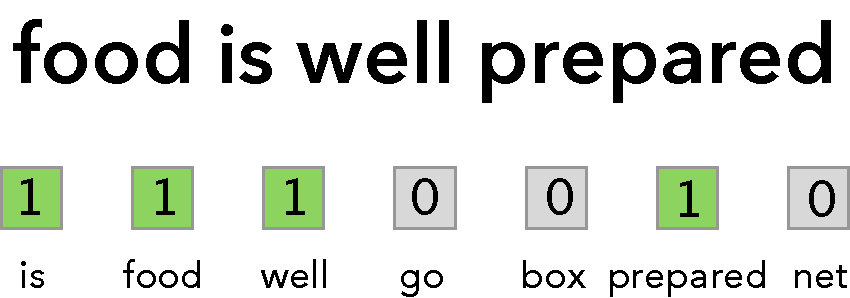
\includegraphics[width=.6\textwidth]{images/bow}}
	\caption{Visualizzazione del modello \emph{bag-of-words}}
	\label{fig:bow}
\end{figure}

\subsection{Architettura della rete}
\label{subsec:modelli1}

Una volta estratte, le features posso essere passate in input alla rete neurale, che le elabora calcolando le risposte dei neuroni dal livello di input verso il livello di output.

In questa prima strategia viene utilizzata una rete \emph{feed-forward} con struttura densa o \emph{fully-connected}. Per i dettagli di queste architetture si rimanda alla Sezione~\ref{subsec:fc}.

Ad ogni livello viene applicata la funzione di attivazione non lineare \emph{ReLU}, descritta nella Sezione~\ref{subsec:fattivazione}.

Inoltre, per accelerare l'apprendimento ed aumentare la stabilità della rete, viene effettuata dopo ogni layer una \emph{Batch Normalization}, definita nella Sezione~\ref{subsec:normalization}. 

Vengono presentate nella tabella \ref{tab:arcbow+fc} tre architetture implementate, con differenti strati e numero di neuroni che caratterizza ciascuno.


\begin{figure}[H]
	\centering
		\begin{tabular}{lcccc}
			\toprule
			\textbf{Layer} \quad & \textbf{Modello 1} & \textbf{Modello 2} & \textbf{Modello 3} \\
			\midrule
			Input 				 & \numprint{60000}	  & \numprint{60000}   &\numprint{60000}\\
			fc1  				 & \numprint{300}		  & 300 		   & {100} 		\\
			fc2  				 &  {200}		  & 200 		   & 50  		\\
			fc3					 & -				  & {100} 		   & 20    	\\
			Output 				 &  {5}			  & {5} 		   & {5}		\\
			\bottomrule
		\end{tabular}
	\captionof{table}{Confronto delle architetture di tre differenti modelli}
	\label{tab:arcbow+fc}
\end{figure}


Tutte le simulazioni sono state addestrate per {10} epoche: la fase di addestramento viene in genere portata avanti fino a quando le performance sul test non producono alcun miglioramento.

L’ottimizzatore scelto è \emph{Adagrad}, introdotto nella Sezione~\ref{subsubsec:adagrad}, con learning rate \numprint{0,001}.

Come funzione di loss è stato scelto l'errore quadratico medio, in inglese \emph{Mean Squared Error (MSE)}, presentato nella Sezione~\ref{subsubsec:MSE}. Mentre la metrica di valutazione utilizzata per misurare le prestazioni predittive del modello è la \emph{Root Mean Squared Error} (RMSE), introdotta nella Sezione~\ref{subsubsec:regressione}.

In ogni epoca si alternano una fase di training ed una fase di test in modo tale da monitorare costantemente i miglioramenti o i peggioramenti del modello sul test set. 

\subsection{Performance}
\label{subsec:performance1}
Prendendo in considerazione le tre diverse architetture implementate, vengono presentati i risultati ottenuti in termini di loss.
\begin{table}[H]
	\centering
	\begin{tabular}{l@{\hspace{.5cm}}ccc}
		\toprule
		 & \textbf{Train loss} & \textbf{Test loss} & \textbf{Tempo di training}  \\
		\midrule
		\textbf{Modello 1} & \numprint{0.061} & \numprint{0.062} &\numprint{235} min \\
		\textbf{Modello 2} & \numprint{0.090} & \numprint{0.061} &\numprint{250} min \\
		\textbf{Modello 3} & \numprint{0.068} & \numprint{0.062} &\numprint{265} min \\
%		\textbf{Modello 4} & \numprint{0.0287} & \numprint{0.0104} &\numprint{145} min \\
		\bottomrule 
	\end{tabular}
	\captionof{table}{Confronto dei risultati in termini di {loss} ottenuti dalle tre diverse reti}
	\label{tab:lossbow+fc}
\end{table}

Per valutare l'efficacia di questi modelli, è fondamentale eseguire un analisi dettagliata, in particolare ponendo l'attenzione sui valori di RMSE per ogni tratto di personalità.
Calcolando il valore medio assunto da ogni caratteristica durante la fase di addestramento, è possibile stabilire qual è il valore di Root Mean Squared Error di un modello concettuale, chiamato ``Modello 0'', che per ogni tratto predice sempre il suo valore medio.
 
\begin{figure}[H]
	\centering
	\begin{tabular}{clccccc}
		\toprule	
		& 		  & \multicolumn{5}{c}{\textbf{Root Mean Squared Error}} 									    \\
		\multicolumn{2}{c}{\multirow{-2}{*}{Modelli}}
		& O 				& C 			   & E 				  & A 				 & N 			    \\ 
		\midrule
		\multirow{2}*{\textbf{Modello 1}} & Modello   & \numprint{0,148} & \numprint{0,227} & \numprint{0,224} & \numprint{0,251} & \numprint{0,351} \\
		& Modello 0 & \numprint{0,145} & \numprint{0,224} & \numprint{0,213} & \numprint{0,218} & \numprint{0,318} \\
		\midrule
		\multirow{2}*{\textbf{Modello 2}} & Modello   & \numprint{0,147} & \numprint{0,226} & \numprint{0,225} & \numprint{0,251} & \numprint{0,341} \\
		& Modello 0 & \numprint{0,141} & \numprint{0,227} & \numprint{0,213} & \numprint{0,208} & \numprint{0,305} \\
		\midrule
		\multirow{2}*{\textbf{Modello 3}} & Modello   & \numprint{0,147} & \numprint{0,226} & \numprint{0,225} & \numprint{0,262} & \numprint{0,348} \\
		& Modello 0 & \numprint{0,233} & \numprint{0,307} & \numprint{0,262} & \numprint{0,373} & \numprint{0,546}  \\
%		\midrule
%		\multirow{2}*{\textbf{Modello 4}} & Modello   & \numprint{0,147} & \numprint{0,22 s6} & \numprint{0,225} & \numprint{0,262} & \numprint{0,348} \\
%		& Modello 0 & \numprint{0,233} & \numprint{0,307} & \numprint{0,262} & \numprint{0,373} & \numprint{0,546}  \\
		\bottomrule	
	\end{tabular}
	\captionof{table}{Confronto dei risultati in termini di {Root Mean Squared Error} delle architetture contro il modello basato sulla media di training}
	\label{tab:confmm0bow+fc}
\end{figure}

\begin{figure}[htb]
	\centering
	{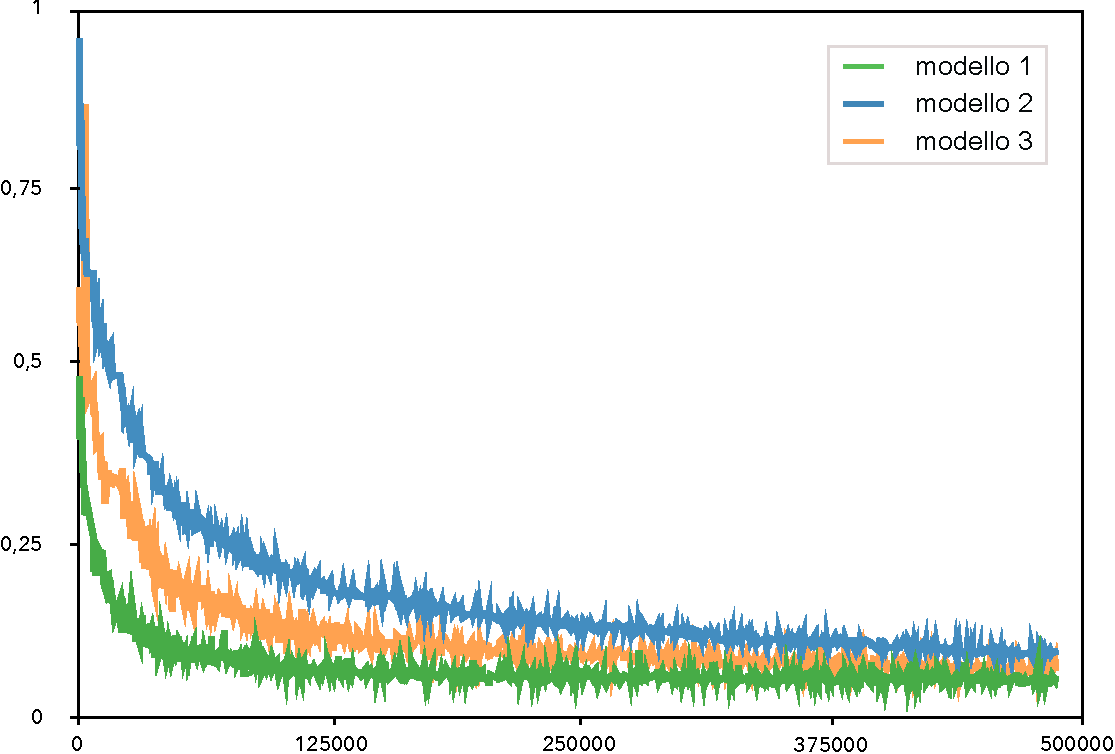
\includegraphics[width=.75\textwidth]{images/loss1}} 
	\caption{Visualizzazione delle training loss dei tre modelli}
	\label{fig:loss}
\end{figure}


Mettendo a confronto le due metriche, si nota che i modelli realmente implementati imparano nella maggioranza dei casi a predire un valore con lo stesso errore commesso dai modelli banali che calcolano la media. Risulta allora evidente che i risultati ottenuti non siano ottimali.

Nonostante ciò, il terzo modello sembrerebbe essere leggermente migliore degli altri due, in particolare confrontandolo con il corrispondente modello nullo si nota la presenza di un piccolo margine di miglioramento.

La scarsa efficienza di questi modelli potrebbe dipendere dall'efficacia con cui vengono codificate le feature in input alla rete. 
Infatti le limitazioni dell'approccio bag-of-words derivano in parte dalla progettazione del vocabolario e della sua dimensione, che può causare una scarsa ``descrizione'' del documento. 
Scartare l'ordine delle parole e ignorare il contesto non consente di determinare la differenza tra le stesse parole disposte diversamente, i sinonimi ecc.
Inoltre, un tipo di rappresentazione sparsa risulta più difficile da modellare quando si cercano modelli in grado di sfruttare poche informazioni in uno spazio rappresentativo ampio, sia per ragioni computazionali (spazio e complessità temporale) sia per ragioni di informazione.

\section{Esperimento 2}
\label{sec:es2}

Durante l'applicazione di tecniche di apprendimento automatico, tutte le ``informazioni'' vengono rappresentate per mezzo di identificativi unici e discreti. 

Nel caso dell'approccio {BoW}, la codifica utilizzata non fornisce alcuna informazione utile al sistema riguardo le relazioni che possono sussistere tra i singoli elementi. Ciò significa che quando sta elaborando i dati, il modello può sfruttare molto poco di ciò che ha appreso su un determinato termine. 

Inoltre la ``raffigurazione'' utilizzata nel precedente esperimento, ha portato alla creazione di dati sparsi. Di conseguenza, per ottenere un modello di successo, un'alternativa valida sarebbe quella di sfruttare {modelli spaziali vettoriali}, in inglese \emph{Vector Space Model} (VSM), per rappresentare le parole in uno spazio continuo \cite{mikolov2013linguistic,erk2008structured}.
Questi metodi dipendono dall'ipotesi distributiva, la quale afferma che le parole che appaiono negli stessi contesti condividono lo stesso significato semantico \cite{baroni2014don}. 

\subsection{Input Features}
\label{subsec:features2}

Nel secondo approccio, viene applicato l'algoritmo non supervisionato \texttt{word2vec} di Tomas Mikolov  \cite{mikolov2013efficient}. 
\texttt{Word2vec} è un modello predittivo particolarmente efficiente dal punto di vista computazionale per l'apprendimento degli embedding di parole a partire dal testo non elaborato.
Esso è basato su una rete neurale artificiale a due strati, addestrati a ricostruire i contesti linguistici delle parole. 

A partire dal corpus di testo, la rete prende in input un set formato dall'accoppiamento di ogni parola target e i contesti in cui appare e restituisce un insieme di vettori che rappresentano la distribuzione semantica delle parole nel testo. 

Viene considerato come ``contesto'' l'insieme delle ``parole a sinistra'' e delle ``parole alla destra'' dell'obiettivo, ovvero la finestra di dimensione 1 attorno all'elemento target. Ogni coppia di destinazione del contesto viene trattata come se fosse una nuova osservazione, incrementando le informazioni distribuzionali. Viene così prodotto uno spazio vettoriale di diverse centinaia di dimensioni, in cui ogni parola univoca viene assegnata a un vettore corrispondente nello spazio.

Per l'implementazione viene utilizzato il modello \emph{skip-gram}, una versione di \texttt{word2vec} che vuole predire le parole del contesto di origine (label) a partire dalle parole target (features).

\begin{figure}[H]
	\centering
	{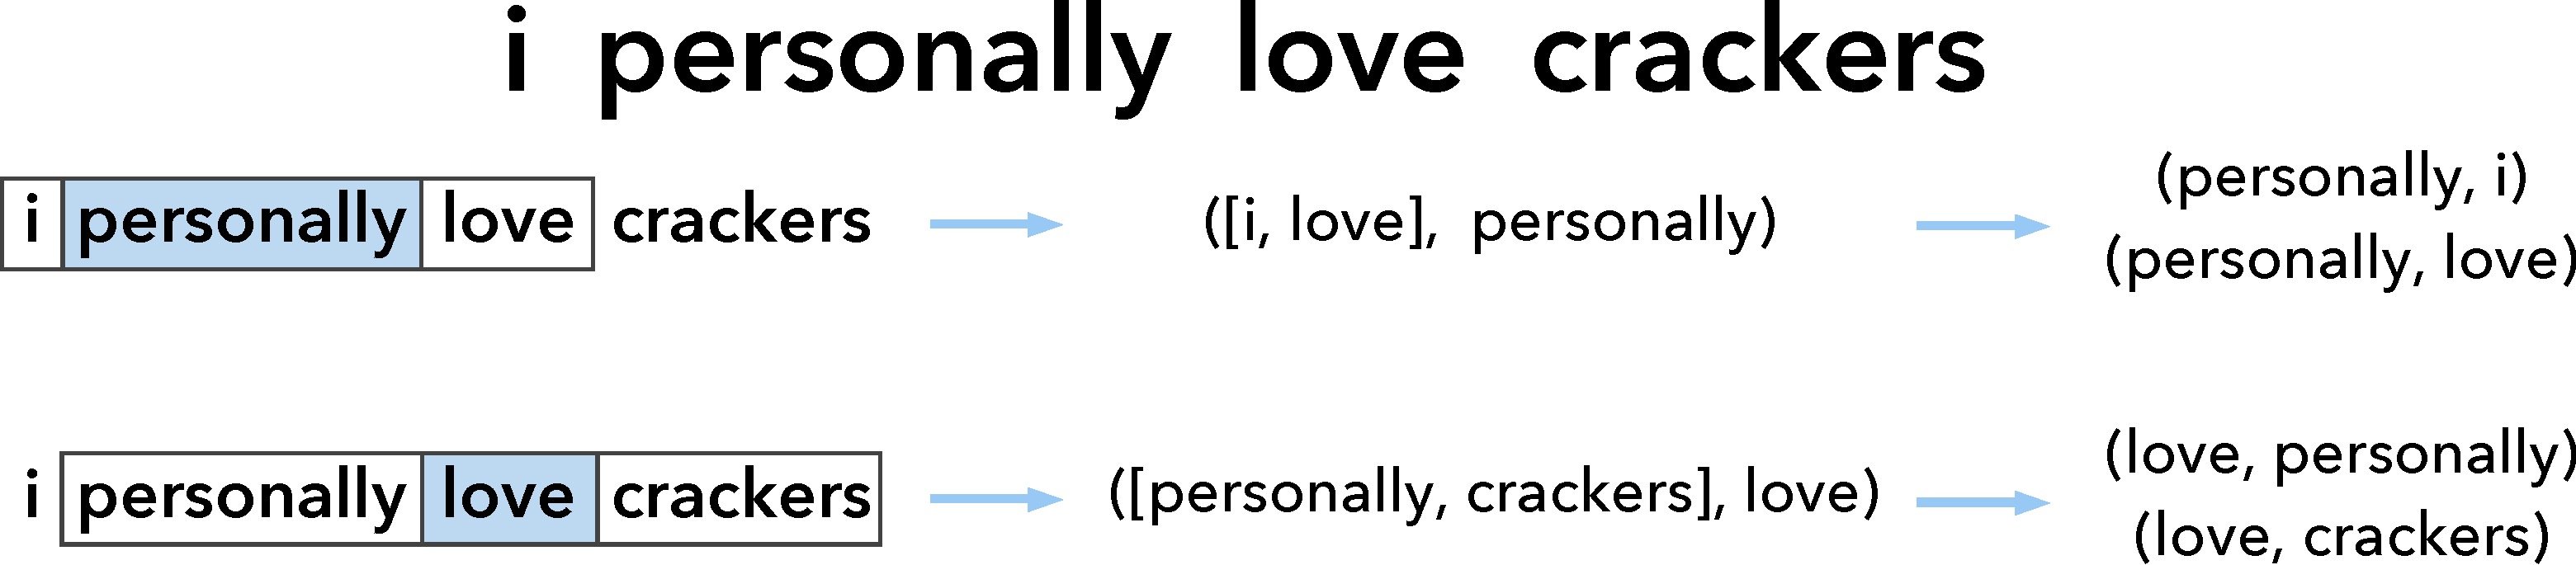
\includegraphics[width=.7\textwidth]{images/skip-gram}} 
	\caption{Visualizzazione del modello skip-gram}
	\label{fig:mikolov}
\end{figure}

In questo tipo di apprendimento, i vettori si posizionano nello spazio in modo tale che le parole che condividono contesti comuni nel corpo siano situate in stretta prossimità l'una dell'altra. Un esempio interessante viene illustrato nella Figura~\ref{fig:embedding1}\subref{subfig:vis3d} --- si ponga particolare attenzione alle parole ``beautiful'', ``lovely'', ``chic'', ``trendy'' ecc.. --- in cui i vocaboli semanticamente simili si trovano vicini dello spazio.

\begin{figure}[H]
	\centering
	\subfloat[][\emph{Visualizzazione 2D}\label{subfig:vis2d}]
	{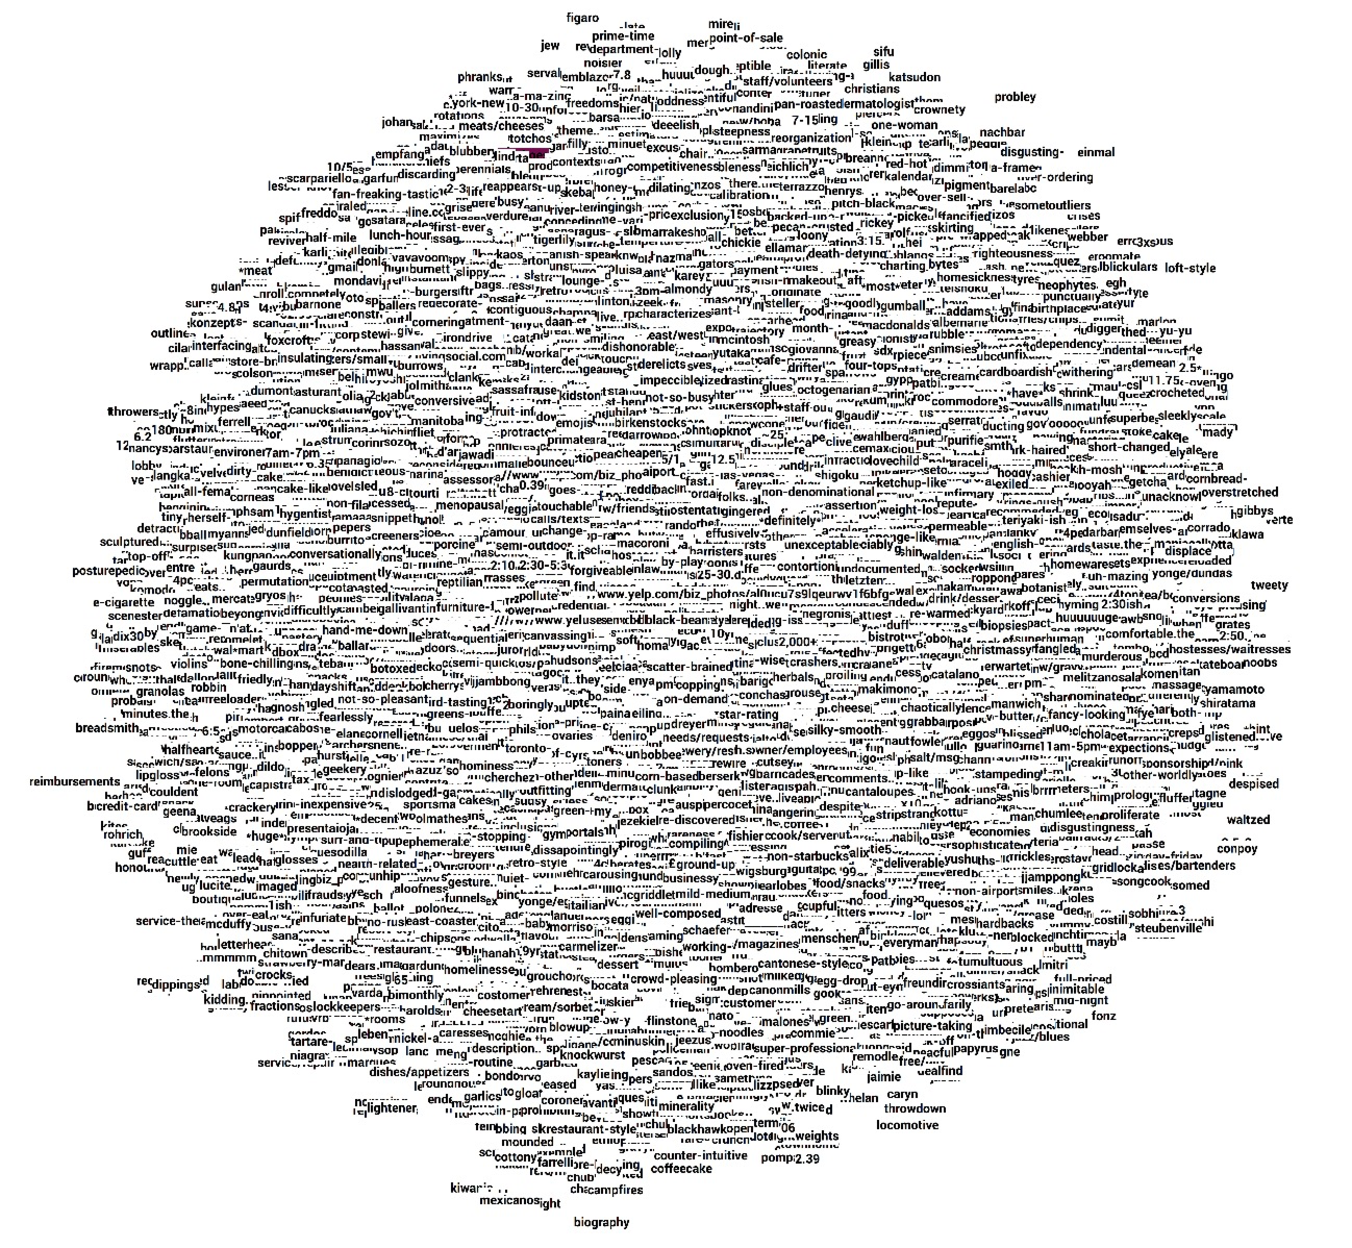
\includegraphics[width=.4\textwidth]{images/embedding1/embedding1_tsne_2d}}
	\hspace{10mm}
	\subfloat[][\emph{Dettaglio di una visualizzazione 3D}\label{subfig:vis3d}]
	{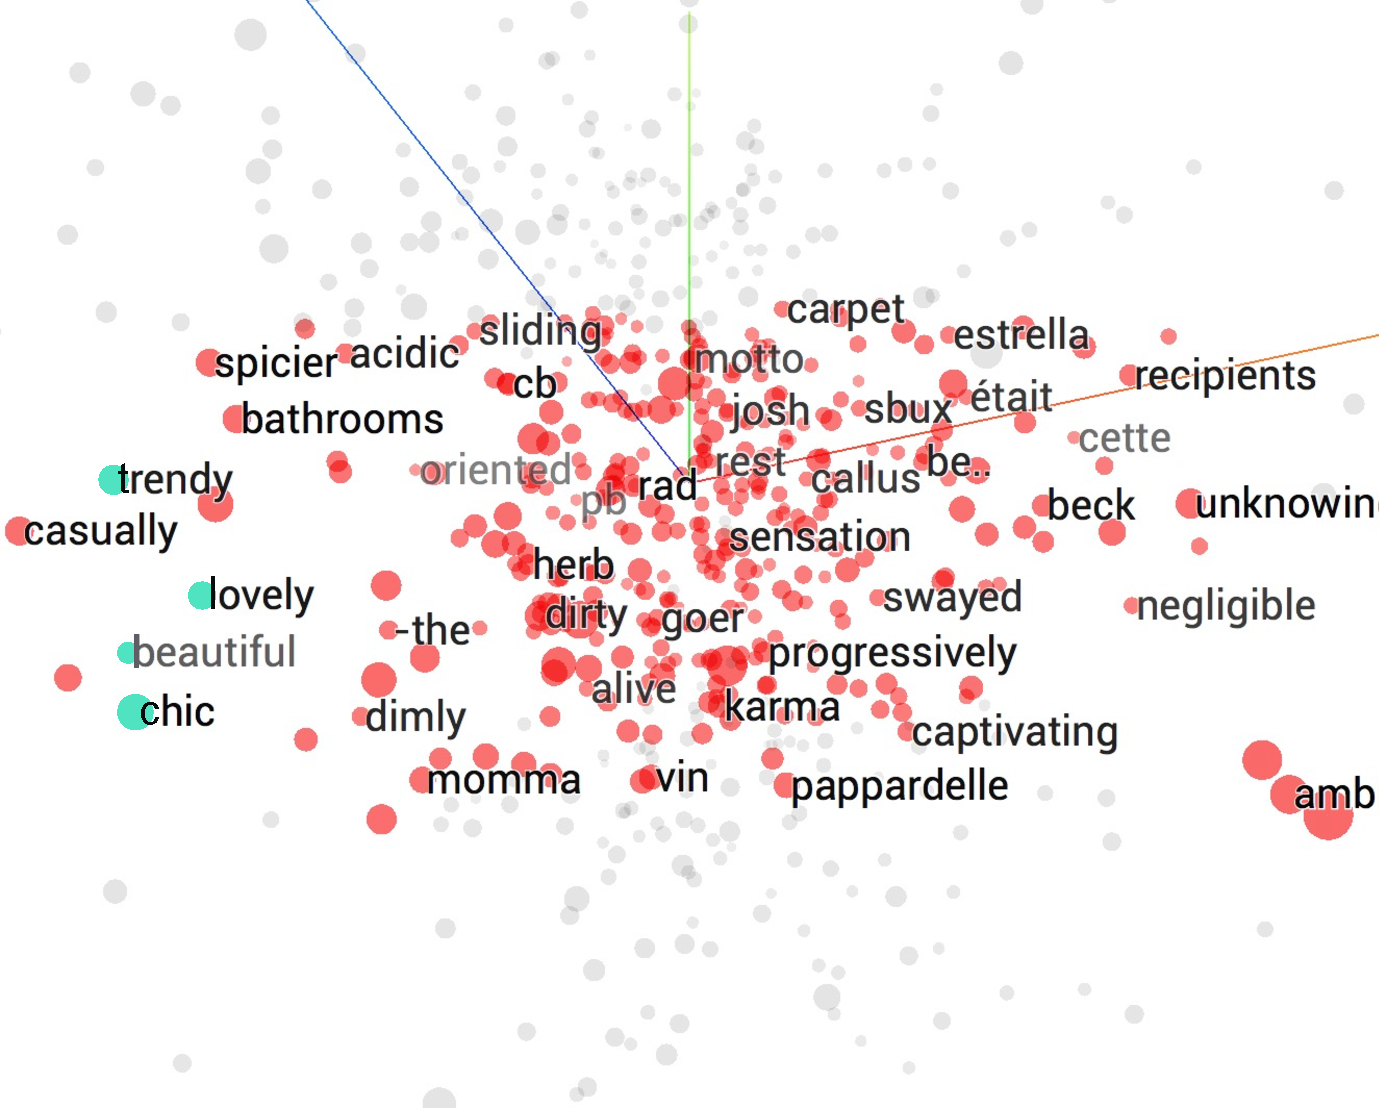
\includegraphics[width=.45\textwidth]{images/embedding1/Embedding1_similarity}}
	
	\caption{Proiezione dell'embedding di Mikolov nello spazio 2-3 dimensionale, tramite la \emph{tecnica di riduzione della dimensionalità} (t-SNE) \cite{maaten2008visualizing}}
	\label{fig:embedding1}
\end{figure}

La funzione obiettivo utilizzata dalla rete per la costruzione dell'embedding viene definita sull'intero set di dati, ed ottimizzata con la \emph{Stochastic Gradient Descent} (SGD), definita nella Sezione~\ref{subsubsec:SGD}.

Nella seguente tabella vengono presentati i due embedding realizzati e i relativi parametri.

\begin{figure}[htb]
	\centering
	\begin{tabular}{ccc}
		\toprule	
		 		  				& \multicolumn{2}{c}{\textbf{Parameters}}	\\
		{\multirow{-2}{*}{Embedding}}
								& Embedding Size 	& Num Sampled 	 		\\ 
		\midrule
		\textbf{Embedding 1}    & \numprint{40} 	& \numprint{20}  		\\
		\midrule
		\textbf{Embedding 2}    & \numprint{250} 	& \numprint{50}  		\\
		\bottomrule	
	\end{tabular}
	\captionof{table}{Confronto dei parametri della rete impostati per la realizzazione dell'embedding}
	\label{tab:confemb}
\end{figure}

\subsection{Architettura della rete}
\label{subsec:modelli2}

La rappresentazione spazio-vettoriale viene utilizzata come feature della modello che si andrà a costruire.
In questo secondo approccio verrà utilizzata un \emph{rete convoluzionale}, in cui ogni neurone è collegato solo a pochi neuroni vicini nel livello precedente, e lo stesso insieme di pesi viene utilizzato per ogni neurone.\\

In questo tipo di rete, il modello di connessione locale e lo schema di peso condiviso possono essere interpretati come un filtro (o un insieme di filtri) che accettano un sottoinsieme dei dati di input alla volta, ma vengono applicati all'intero input.

Uno strato convoluzionale è molto più specializzato ed efficiente di uno completamente connesso.

\begin{figure}[H]
	\centering
	{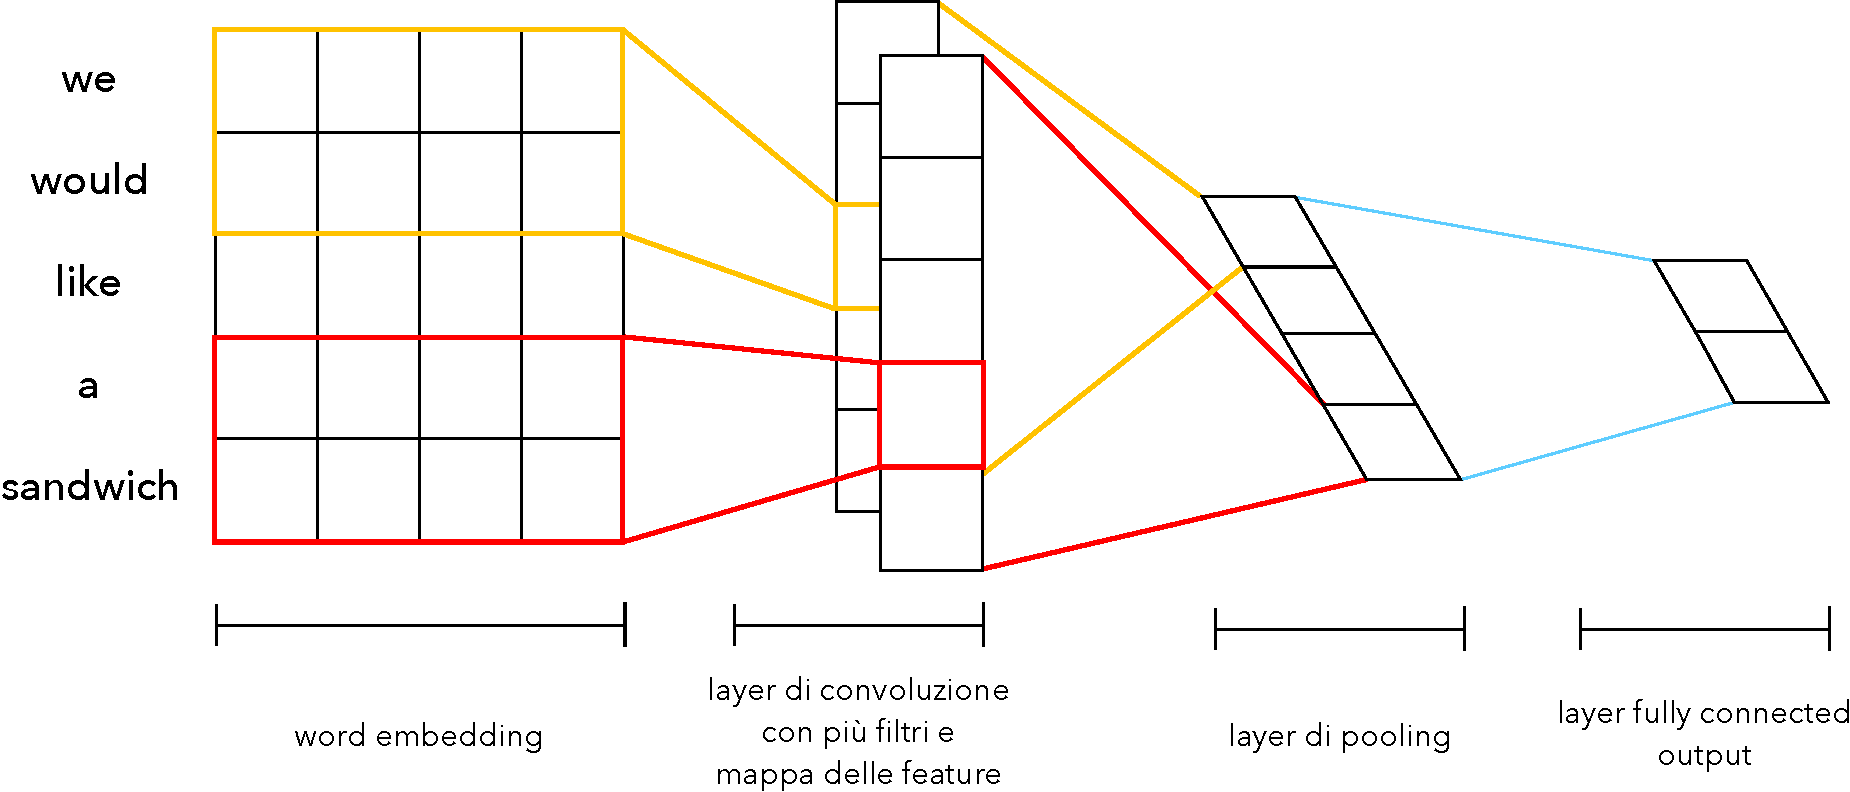
\includegraphics[width=.85\textwidth]{images/cnn}} 
	\caption{Esempio di architettura convoluzionale per la manipolazione del linguaggio naturale}
	\label{fig:cnn}
\end{figure}

Le operazioni eseguite da questi strati vengono trasformate in ``moltiplicazioni'' non lineari tramite l'applicazione della funzione di attivazione \emph{ReLU}, introdotta nella Sezione~\ref{subsec:fattivazione}.

Ad ogni livello convoluzionale viene applicata una \emph{Batch Normalization}, definita nella Sezione~\ref{subsec:normalization}, utilizzata sull'input per il ridimensionamento delle funzionalità e la normalizzazione batch nei livelli nascosti.

Dopo il primo strato convoluzionale viene inserito un \emph{layer di pooling}, introdotto nella Sezione~\ref{subsec:maxpool}, necessario per ridurre in modo efficace i campioni dell'output del livello precedente, riducendo il numero di operazioni richieste per tutti i livelli successivi, ma passando comunque le informazioni valide.

Come ultimo strato della rete viene scelto un \emph{layer fully-connected}, definito nella Sezione~\ref{subsec:fc}, corrispondente ad un'operazione lineare sul vettore di input del livello che esegue una serie di trasformazioni sulla rappresentazione profonda al fine di emettere i punteggi di ogni classe.

\begin{figure}[H]
	\centering
	\begin{tabular}{lccc}
		\toprule
		\textbf{Layer}& \textbf{Modello 4} & \textbf{Modello 5} & \textbf{Modello 6} 		\\ 
		\midrule
		conv1 	& {10}$\times${5}, 10	  & {5}$\times${5}, 150, same pad    &{3}$\times${3}, 100, same pad 		   \\
		
		mpool1 	& &{{4}$\times${4}, stride 2, same pad}	&   \\
		conv2  	& {18}$\times${18}, 10	  &  {5}$\times${20}, 100, same pad	  &		{3}$\times${20}, 75, same pad    \\
		conv3  	& ---	  & {1}$\times${20}, 50, 	   &	{1}$\times${20}, 50 	   \\
		fcout		& &{{1}$\times${1}, 5}&		   \\
		
		\bottomrule	
	\end{tabular}
	\captionof{table}{Architetture implementate a partire dall'embedding 1}
	\label{tab:netemb1}
\end{figure}

\begin{figure}[H]
	\centering
	\begin{tabular}{lcc}
		\toprule
		\textbf{Layer}& \textbf{Modello 7} 								  & \textbf{Modello 8} 			   \\ 
		\midrule
		conv1 	& {3}$\times${3}, 100, stride 2, same pad     & ---	   \\
		mpool1 	& {4}$\times${4}, stride 2, same pad		  & ---	   \\
		conv2  	& {3}$\times${63}, 75, stride 2, same pad	  & ---    \\
		conv3  	& {1}$\times${32}, 50, stride 2	  				  & ---	   \\
		fc1  	& ---													  & {1}$\times${1}, 100	   \\
		fc2  	& {1}$\times${32}, 50, stride 2	  				  & {1}$\times${1},  50    \\
		fc3  	& {1}$\times${32}, 50, stride 2	  				  & {1}$\times${1},  20	   \\
		fcout	& {1}$\times${1}, 5   			  				  & {1}$\times${1},   5	   \\
		\bottomrule	
	\end{tabular}
	\captionof{table}{Architetture implementate a partire dall'embedding 2}
	\label{tab:netemb2}
\end{figure}

Vengono presentate nelle tabelle \ref{tab:netemb1} e \ref{tab:netemb2} le diverse configurazioni dei layer convoluzionali delle architetture implementate per i due embedding.\\

L'input della rete è costituito da un numero di caratteristiche pari a $n \times p$ dove $n$ è la dimensione dell'embedding e $p$ il numero delle parole di ogni sentence.

Come algoritmo di ottimizzazione viene scelto sempre \emph{Adagrad}, illustrato nella Sezione~\ref{subsubsec:adagrad}, mentre il valore di \emph{learning rate} settato per ogni modello viene mostrato nella tabella \ref{tab:learningratemikolov}.

Viene mantenuta anche in questa simulazione la funzione di costo MSE, approfondita nella Sezione~\ref{subsubsec:MSE}.

Nel caso del secondo embedding si è voluto provare anche un modello che sfruttasse solo livelli di rete \emph{fully-connected}, senza applicare alcuna convoluzione. 


\begin{table}[t]
	\centering
	\begin{tabular}{llc}
		\toprule
		\multicolumn{2}{c}{{Modelli}} & \textbf{Learning Rate}  \\
		\midrule
		\multirow{3}*{{Embedding 1}} 
		&\textbf{Modello 4} & \numprint{0.0010} \\
		&\textbf{Modello 5} & \numprint{0.0001} \\
		&\textbf{Modello 6} & \numprint{0.0050} \\
		\midrule
		\multirow{2}*{{Embedding 2}} 
		&\textbf{Modello 7} & \numprint{0.0050} \\
		&\textbf{Modello 8} & \numprint{0.0001} \\	
		\bottomrule 
	\end{tabular}
	\captionof{table}{Learning rate delle simulazioni effettuate nell'esperimento 2}
	\label{tab:learningratemikolov}
\end{table}

\subsection{Performance}
\label{subsec:performance2}

Prendendo in considerazione i due diversi embedding, vengono messe a confronto a confronto le diverse architetture implementate, mostrando i risultati ottenuti in termini di loss.
\begin{table}[H]
	\centering
	\begin{tabular}{ll@{\hspace{.5cm}}ccc}
		\toprule
		\multicolumn{2}{c}{{Modelli}} & \textbf{Train loss} & \textbf{Test loss} & \textbf{Tempo di training}  \\
		\midrule
		\multirow{3}*{{Embedding 1}} 
		&\textbf{Modello 4} & \numprint{0.061} & \numprint{0.058} &\numprint{200} min \\
		&\textbf{Modello 5} & \numprint{0.052} & \numprint{0.060} &\numprint{310} min \\
		&\textbf{Modello 6} & \numprint{0.042} & \numprint{0.060} &\numprint{540} min \\
		\midrule
		\multirow{2}*{{Embedding 2}} 
		&\textbf{Modello 7} & \numprint{0.038} & \numprint{0.057} &\numprint{225} min \\
		&\textbf{Modello 8} & \numprint{0.058} & \numprint{0.117} &\numprint{250} min \\	
		\bottomrule 
	\end{tabular}
	\captionof{table}{Confronto dei risultati in termini di \emph{loss} ottenuti nelle diverse reti con i due diversi embedding}
	\label{tab:lossmikolov}
\end{table}

Valutando le prestazioni su train e test set viene rilevato il ``Modello 7'' come il migliore tra quelli proposti, presentando i valori di loss più bassi. 
Oltre a ciò, anche rispetto al precedente approccio il ``Modello 7'' mostra una performance migliorata circa 
del $3\%$.

Vengono analizzati anche i valori di RMSE, relativi ad ogni tratto di personalità, riassunti nella tabella \ref{tab:rmsemikolov}, e viene inoltre visualizzata la curva RMSE nella Figura~\ref{fig:rmse}.

\begin{figure}[H]
	\centering
	{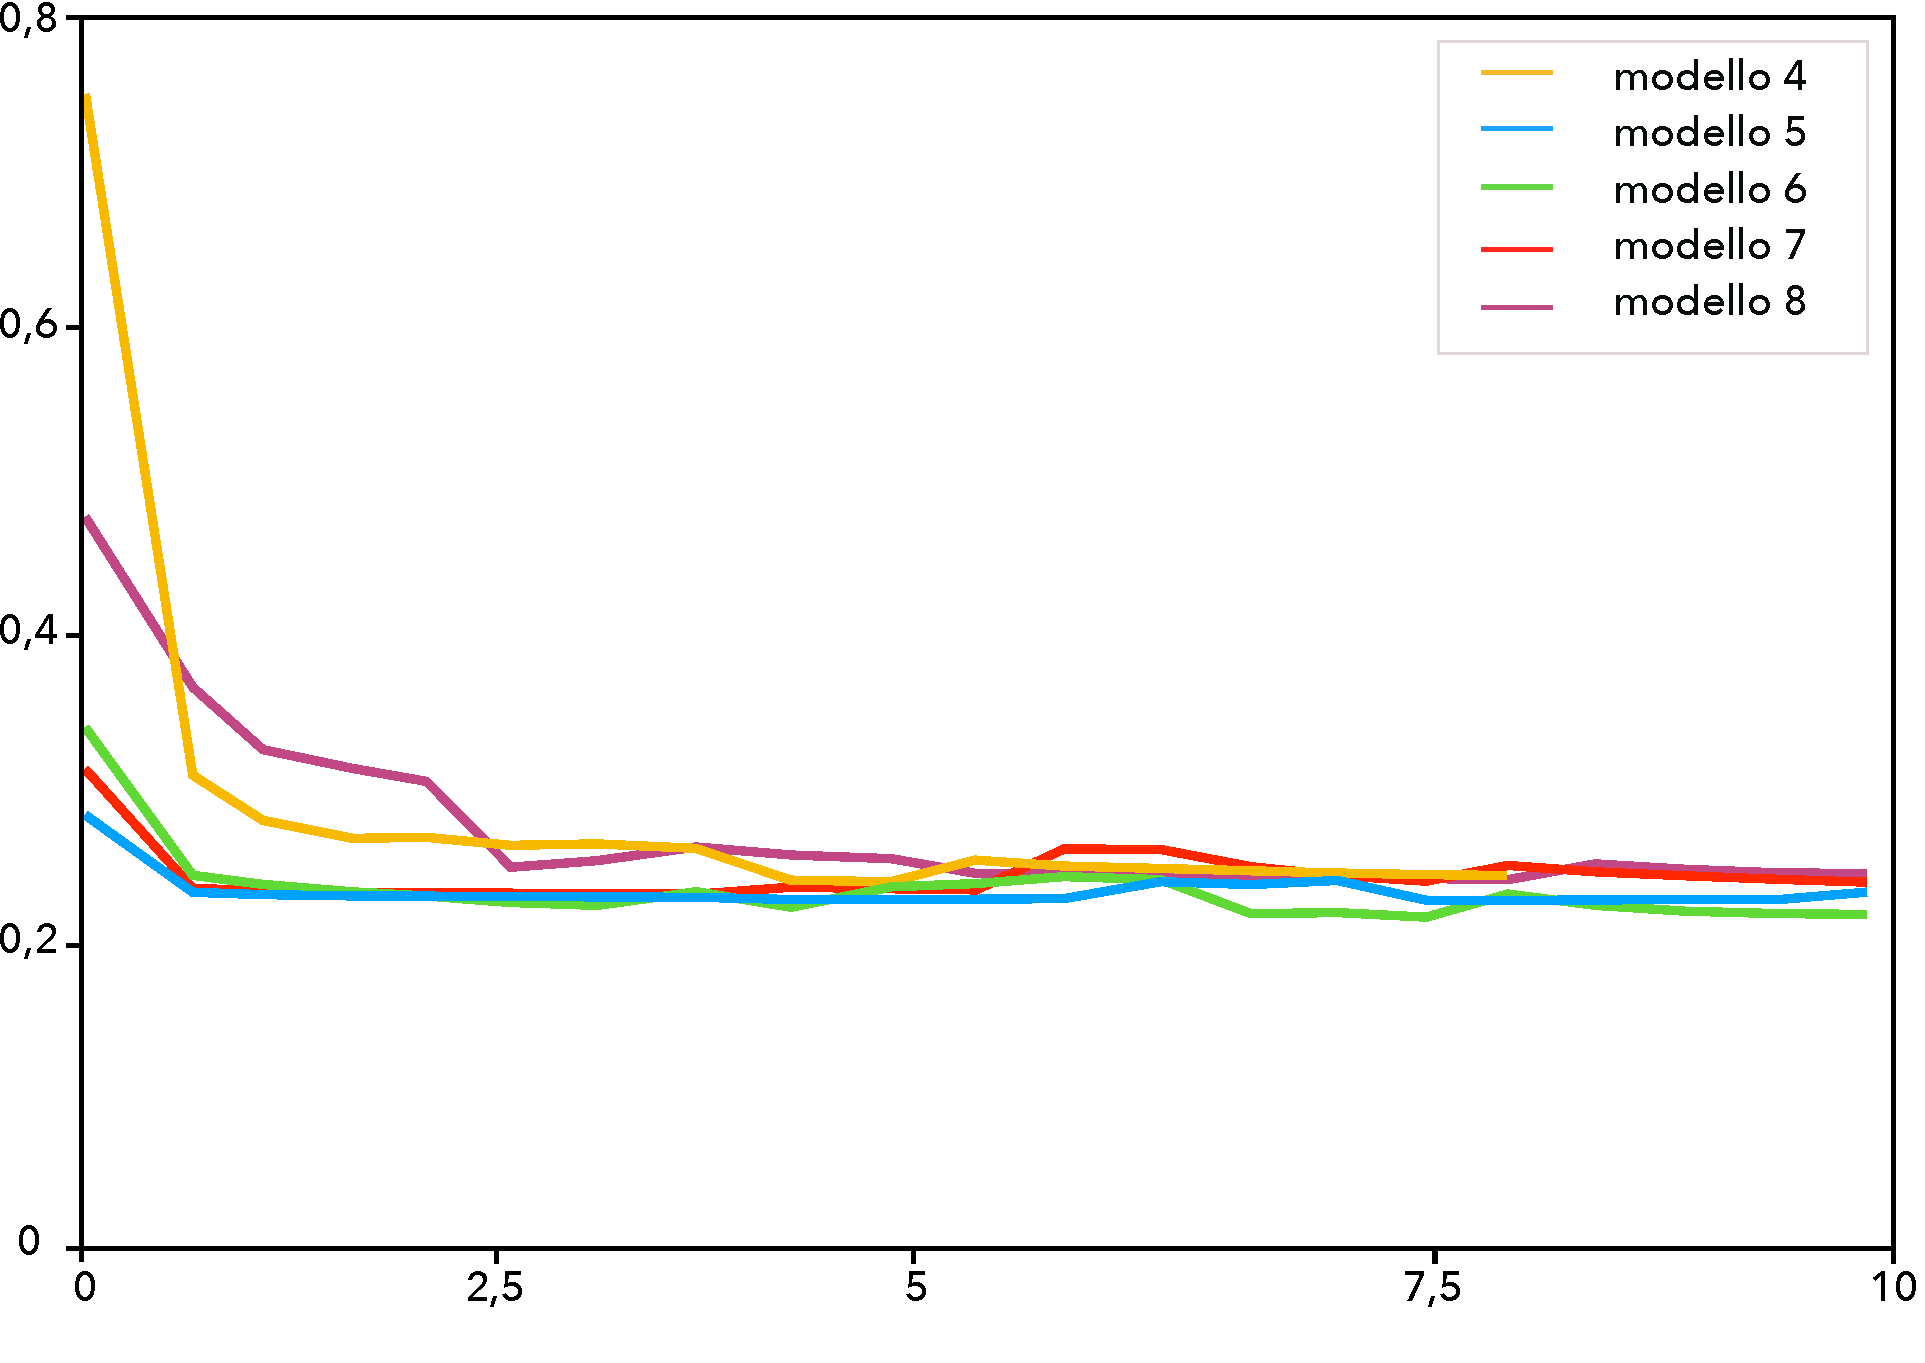
\includegraphics[width=.65\textwidth]{images/rmse2-linlong}} 
	\caption{Visualizzazione delle training RMSE dei modelli}
	\label{fig:rmse}
\end{figure}

\begin{figure}[t]
	\centering
	\begin{tabular}{clccccc}
		\toprule	
		& 		 			& \multicolumn{5}{c}{\textbf{Root Mean Squared Error}} 									       \\
		\multicolumn{2}{c}{\multirow{-2}{*}{Modelli}}
		& O 				& C 			   & E 				  & A 				 & N 			   \\ 
		\midrule
		\multirow{3}*{{Embedding 1}} 
		& \textbf{Modello 4} & \numprint{0,148} & \numprint{0,226} & \numprint{0,232} & \numprint{0,252} & \numprint{0,313} \\
		& \textbf{Modello 5} & \numprint{0,146} & \numprint{0,227} & \numprint{0,230} & \numprint{0,251} & \numprint{0,336} \\
		& \textbf{Modello 6} & \numprint{0,146} & \numprint{0,225} & \numprint{0,224} & \numprint{0,251} & \numprint{0,337} \\
		\midrule
		\multirow{2}*{{Embedding 2}} 
		& \textbf{Modello 7} & \numprint{0,147} & \numprint{0,223} & \numprint{0,222} & \numprint{0,251} & \numprint{0,320} \\
		& \textbf{Modello 8} & \numprint{0,399} & \numprint{0,275} & \numprint{0,257} & \numprint{0,271} & \numprint{0,457} \\
		\bottomrule	
	\end{tabular}
	\captionof{table}{Confronto dei risultati in termini di {Root Mean Squared Error} delle architetture sul test set}
	\label{tab:rmsemikolov}
\end{figure}


\section{Esperimento 3}
\label{sec:es3}

Nel terzo approccio si decide di valutare una rappresentazione dell'input alternativa.

\subsection{Input Features}
\label{subsec:features3}

Ricorrendo nuovamente al modello \emph{skip-gram}, l'input della rete questa volta comprende il set formato dall'accoppiamento tra gli aggettivi contenuti nel dizionario OCEAN e i loro contesti.

La finestratura che si andrà a definire in torno al target sarà di dimensione 2 e considererà le due parole a sinistra e le due parole a destra dell'aggettivo. La window non sarà più quindi incentrata su ogni elemento della sentence.
Dunque nell'embedding che si andrà a costruire non verranno appresi i contesti di tutte le parole, ma solamente quelli di nostro interesse, ovvero relativi agli aggettivi.

In questo esperimento viene realizzato un solo embedding, la cui dimensione è {250} e con numero di etichette negative da campionare pari a 50 \cite{liu2016classification}.

\subsection{Architettura della rete}
\label{subsec:modelli3}

Viene utilizzato l'embedding estratto per costruire due modelli di reti neurali, le cui architetture vengono presentate nella tabella \ref{tab:netemb3}.
Come nel precedente esperimento si ricorrerà alle \emph{reti convoluzionali}; si rimanda alla Sezione~\ref{subsec:modelli2} per i dettagli. 

\begin{figure}[H]
	\centering
	\begin{tabular}{lcc}
		\toprule
		\textbf{Layer}& \textbf{Modello 9} & \textbf{Modello 10}	\\ 
		\midrule
		conv1   & {7}$\times${5}, 100, stride 2, same pad    		&{3}$\times${3}, 100, stride 2, same pad 		   \\
		mpool1 	&\multicolumn{2}{c}{{4}$\times${4}, stride 2, same pad}	 \\
		conv2  	&  {5}$\times${63}, 75, stride 2, same pad	    &		{3}$\times${63}, 75, stride 2, same pad    \\
		conv3  	& {3}$\times${32}, 50, stride 2, same pad 	   	&	{1}$\times${32}, 50, stride 2 	   \\
		conv4  	& {1}$\times${16}, 25, stride 2 	   	&	--- 	   \\
		fcout	&\multicolumn{2}{c}{{1}$\times${1}, 5}						\\
		
		\bottomrule	
	\end{tabular}
	\captionof{table}{Architetture dei due modelli implementati a partire dall'embedding 3}
	\label{tab:netemb3}
\end{figure}

L'algoritmo di apprendimento utilizzato è \emph{Adagrad}, definito nella Sezione~\ref{subsubsec:adagrad}, con \emph{learning rate} \numprint{0,0005} per il ``Modello 9'' e \numprint{0,005} per il ``Modello 10''. La funzione di \emph{loss} scelta è la MSE, introdotta nella Sezione~\ref{subsubsec:MSE}. 

\subsection{Performance}
\label{subsec:performance3}

Vengono presentati nella tabella \ref{tab:lossmikolov2} i valori ottenuti dalla funzione obiettivo dei due modelli, mentre nella tabella \ref{tab:rmsemikolov2} vengono riassunti i valori di RMSE per ogni tratto di personalità.

\begin{table}[H]
	\centering
	\begin{tabular}{l@{\hspace{.5cm}}ccc}
		\toprule
		& \textbf{Train loss} & \textbf{Test loss} & \textbf{Tempo di training}  \\
		\midrule
		\textbf{Modello 9} & \numprint{0.043} & \numprint{0.060} &\numprint{18} h \\
		\textbf{Modello 10} & \numprint{0.050} & \numprint{0.059} &\numprint{17} h \\	
		\bottomrule 
	\end{tabular}
	\captionof{table}{Confronto dei risultati in termini di {loss} ottenuti nell'implementazione dei due modelli}
	\label{tab:lossmikolov2}
\end{table}

\begin{figure}[H]
	\centering
	\begin{tabular}{clccccc}
		\toprule	
		& 		 			& \multicolumn{5}{c}{\textbf{Root Mean Squared Error}} 									       \\
		\multicolumn{2}{c}{\multirow{-2}{*}{Modelli}}
		& O 				& C 			   & E 				  & A 				 & N 			   \\ 
		\midrule
		& \textbf{Modello 9} & \numprint{0,146} & \numprint{0,223} & \numprint{0,223} & \numprint{0,251} & \numprint{0,331} \\
		& \textbf{Modello 10} & \numprint{0,147} & \numprint{0,225} & \numprint{0,224} & \numprint{0,252} & \numprint{0,339} \\
		\bottomrule	
	\end{tabular}
	\captionof{table}{Confronto dei risultati in termini di {RMSE} delle due architetture sul test set}
	\label{tab:rmsemikolov2}
\end{figure}

Rispetto al precedente approccio non vengono ottenuti dei miglioramenti. 

\section{Esperimento 4}
\label{sec:es4}

L'ultimo approccio provato riutilizza i precedenti metodi di estrazione di feature che hanno ottenuto le migliori prestazioni per realizzare un modello predittivo di classificazione.

Nello specifico il problema viene trasformato in un compito di classificazione binaria multi-label, in cui si cercano di predire cinque diverse etichette per ogni istanza. 

Per ogni dimensione di personalità l'output della rete sarà ``0'', se il valore reale che assume un determinato tratto è inferiore a 0, o ``1'' altrimenti.
\\
Viene stabilito 0 come ``punto di neutralità assoluta'' perché corrisponde alla media dei valori osservati in ognuna delle caratteristiche.

Adottando questo metodo, si assumerà di poter estrarre da questa funzione una misura di polarità, positiva o negativa, che indicherà un tratto più o meno accentuato.

Il vantaggio effettivo di questo approccio consiste nella possibilità di valutare le performance in modo standard, visualizzando le matrici di confusione e misurandone l'accuratezza, argomenti trattati nella Sezione~\ref{subsubsec:classificazione}.

\subsection{Input Features}
\label{subsec:features4}

Vengono utilizzati come ingresso della rete due embedding di Mikolov realizzati negli esperimenti precedenti, ovvero l'``Embedding 2'' e l'``Embedding 3''.

\subsection{Architettura della rete}
\label{subsec:modelli4}

Le reti che vengono realizzate sono molto simili a quelle precedentemente implementate; i dettagli delle architetture vengono presentati nella tabella \ref{tab:netemb4}.

Ad ogni livello della rete viene applicata la stessa procedura degli esperimenti precedenti. 

\begin{figure}[H]
	\centering
	\begin{tabular}{lccc}
		\toprule
		\textbf{Layer} & \textbf{Modello 11} & \textbf{Modello 12} & \textbf{Modello 13}  	\\ 
		\midrule
		conv1 	& {3}$\times${3}, 100	  & {5}$\times${3}, 100 & {7}$\times${5}, 100 	   \\
		mpool1 	& {{4}$\times${4}}	&{{4}$\times${4}}	& {{4}$\times${4}}	 \\
		conv2  	& {3}$\times${63}, 75 &  {3}$\times${63}, 75	  &		{5}$\times${63}, 75    \\
		conv3  	&{1}$\times${32}, 50	  & {1}$\times${32}, 50  &	{3}$\times${32}, 50 	  \\
		conv4  	& ---	  & {1}$\times${16}, 25  &	{1}$\times${16}, 25 	  \\
		fcout	&{{1}$\times${1}, 10} &{{1}$\times${1}, 10}&{{1}$\times${1}, 10}		   \\
		\bottomrule	
	\end{tabular}
	\captionof{table}{Architetture implementate a partire dall'embedding 2}
	\label{tab:netemb4}
\end{figure}

In ogni livello convoluzionale della rete si utilizzano uno stride di dimensione 2 e padding same, tranne che per l'ultimo livello convoluzionale con padding valid, per i dettagli si consiglia di visitare la sezione { \ref{subsec:cnn}}.

\begin{figure}[H]
	\centering
	\begin{tabular}{lcc}
		\toprule
		\textbf{Layer} & \textbf{Modello 14} & \textbf{Modello 15}   	\\ 
		\midrule
		conv1 	& {{7}$\times${5}, 100, stride 2, same pad}&{{7}$\times${5}, 100, stride 2, same pad} \\
		mpool1 	& {{4}$\times${4}, stride 2, same pad} &{{4}$\times${4}, stride 2, same pad}  \\
		conv2  	& {{5}$\times${63}, 75, stride 2, same pad}&{{5}$\times${63}, 75, stride 2, same pad}    \\
		conv3  	&  {{3}$\times${32}, 50, stride 2, same pad} &{{3}$\times${32}, 50, stride 2, same pad} 	  \\
		conv4  	& {1}$\times${16}, 25, stride 2  &	{3}$\times${16}, 25, stride 2, same pad 	  \\
		conv5  	& ---  &	{1}$\times${8}, 16, stride 2 	  \\
		fcout	& \multicolumn{2}{c}{{1}$\times${1}, 10}		   \\
		\bottomrule	
	\end{tabular}
	\captionof{table}{Architetture implementate a partire dall'embedding 3}
	\label{tab:rmsebin2}
\end{figure}

In tutte le simulazioni l’ottimizzatore scelto è \emph{Adagrad}, introdotto nella Sezione~\ref{subsubsec:adagrad}, il valore di \emph{learning rate}  di ogni modello viene mostrato nella tabella \ref{tab:learningratemikolov2}.

Come funzione obiettivo viene utilizzata la \emph{Softamax Cross Entropy}, presentata nella Sezione~\ref{subsubsec:sce}. 

\begin{table}[H]
	\centering
	\begin{tabular}{llc}
		\toprule
		\multicolumn{2}{c}{{Modelli}} & \textbf{Learning Rate}  \\
		\midrule
		\multirow{3}*{{Embedding 2}} 
		&\textbf{Modello 11} & \numprint{0.0001} \\
		&\textbf{Modello 12} & \numprint{0.0005} \\
		&\textbf{Modello 13} & \numprint{0.0005} \\
		\midrule
		\multirow{2}*{{Embedding 3}} 
		&\textbf{Modello 14} & \numprint{0.0005} \\
		&\textbf{Modello 15} & \numprint{0.0005} \\	
		\bottomrule 
	\end{tabular}
	\captionof{table}{Learning rate delle simulazioni effettuate nell'esperimento 2}
	\label{tab:learningratemikolov2}
\end{table}


\subsection{Performance}
\label{subsec:performance4}

Prendendo in considerazione le diverse architetture implementate, vengono presentati i risultati ottenuti in termini di loss.

\begin{table}[H]
	\centering
	\begin{tabular}{ll@{\hspace{.5cm}}ccc}
		\toprule
		\multicolumn{2}{c}{{Modelli}} & \textbf{Train loss} & \textbf{Test loss} & \textbf{Tempo di training}  \\
		\midrule
		\multirow{3}*{{Embedding 2}} 
		&\textbf{Modello 11} & \numprint{3.275} & \numprint{3.455} &\numprint{20} h \\
		&\textbf{Modello 12} & \numprint{3.297} & \numprint{3.459} &\numprint{30} h \\
		&\textbf{Modello 13} & \numprint{3.444} & \numprint{3.458} &\numprint{40} h \\
		\midrule
		\multirow{2}*{{Embedding 2}} 
		&\textbf{Modello 14} & \numprint{3.350} & \numprint{3.459} &\numprint{20} h \\
		&\textbf{Modello 15} & \numprint{3.230} & \numprint{3.454} &\numprint{60} h \\	
		\bottomrule 
	\end{tabular}
	\captionof{table}{Confronto delle \emph{loss} ottenute nelle diverse reti con i due diversi embedding}
	\label{tab:lossmikolov3}
\end{table}

Come già detto, l'utilizzo di questo approccio consente una valutazione non più solo in termini di loss ma se ne potrà analizzare anche l'accuratezza, introdotta nella Sezione~\ref{subsubsec:classificazione}. 

\begin{figure}[H]
	\centering
	\begin{tabular}{clP{1cm}P{1cm}P{1cm}P{1cm}P{1cm}}
		\toprule	
		& 		 			& \multicolumn{5}{c}{\textbf{Train/Test Accuracy [\%]} 		}							       \\
		\multicolumn{2}{c}{\multirow{-2}{*}{Modelli}}
		& O 				& C 			   & E 				  & A 				 & N 			   \\ 
		\midrule
		\multirow{3}*{{Embedding 2}} 
		& \textbf{Modello 11} & \numprint{61}/\numprint{61} & \numprint{60}/\numprint{59} & \numprint{63}/\numprint{60} & \numprint{58}/\numprint{56} & \numprint{57}/\numprint{54} \\
		
		& \textbf{Modello 12} &\numprint{62}/\numprint{59} &\numprint{61}/\numprint{50} & \numprint{64}/\numprint{45} & \numprint{61}/\numprint{56} & \numprint{61}/\numprint{56} \\
		
		& \textbf{Modello 13} & \numprint{63}/\numprint{55} &\numprint{63}/\numprint{60} & \numprint{63}/\numprint{61} & \numprint{63}/\numprint{58} & \numprint{62}/\numprint{59} \\
		\midrule
		\multirow{2}*{{Embedding 3}} 
		& \textbf{Modello 14} & \numprint{61}/\numprint{61} & \numprint{61}/\numprint{57} & \numprint{62}/\numprint{52} & \numprint{60}/\numprint{57} & \numprint{60}/\numprint{56} \\
		
		& \textbf{Modello 15} &\numprint{63}/\numprint{60} & \numprint{62}/\numprint{48} & \numprint{64}/\numprint{60} & \numprint{62}/\numprint{49} & \numprint{62}/\numprint{48} \\
		\bottomrule	
	\end{tabular}
	\captionof{table}{Confronto delle accuracy sul test set delle diverse architetture}
	\label{tab:accuracymikolov}
\end{figure}

Il ``Modello 13'' sembrerebbe il migliore tra quelli proposti poiché presenta valori di accuracy più alti e la differenza di prestazioni tra train e test set è una tra le più basse, dimostrando minore propensione all'overfitting.  \\

Viene presentata un analisi più dettagliata su questo modello, in particolare mostrando il grafico dell'accuratezza, su train e test set, e le matrici di confusione calcolate per ogni tratto di personalità.

Come si può vedere chiaramente dalle matrici di confusione, le caratteristiche \emph{Conscientiousness} e \emph{Extraversion} sono quelle che vengono predette nel modo peggiore.

\begin{figure}[H]
	\centering
	\subfloat[][\emph{Visualizzazione matrice di confusione}\label{subfig:confO}]{
		\begin{minipage}[c][0.7\width]{0.45\textwidth}
			\centering
			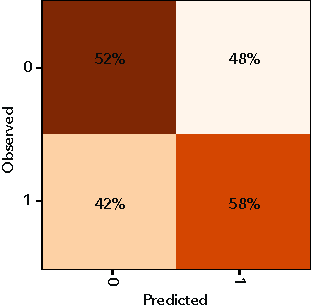
\includegraphics[width=.6\textwidth]{images/binary/accO}
		\end{minipage}} 
	\hspace{10mm}
	\subfloat[][\emph{Visualizzazione accuratezza su train e test}\label{subfig:accO}]{
		\begin{minipage}[c][0.7\width]{0.45\textwidth}
			\centering
			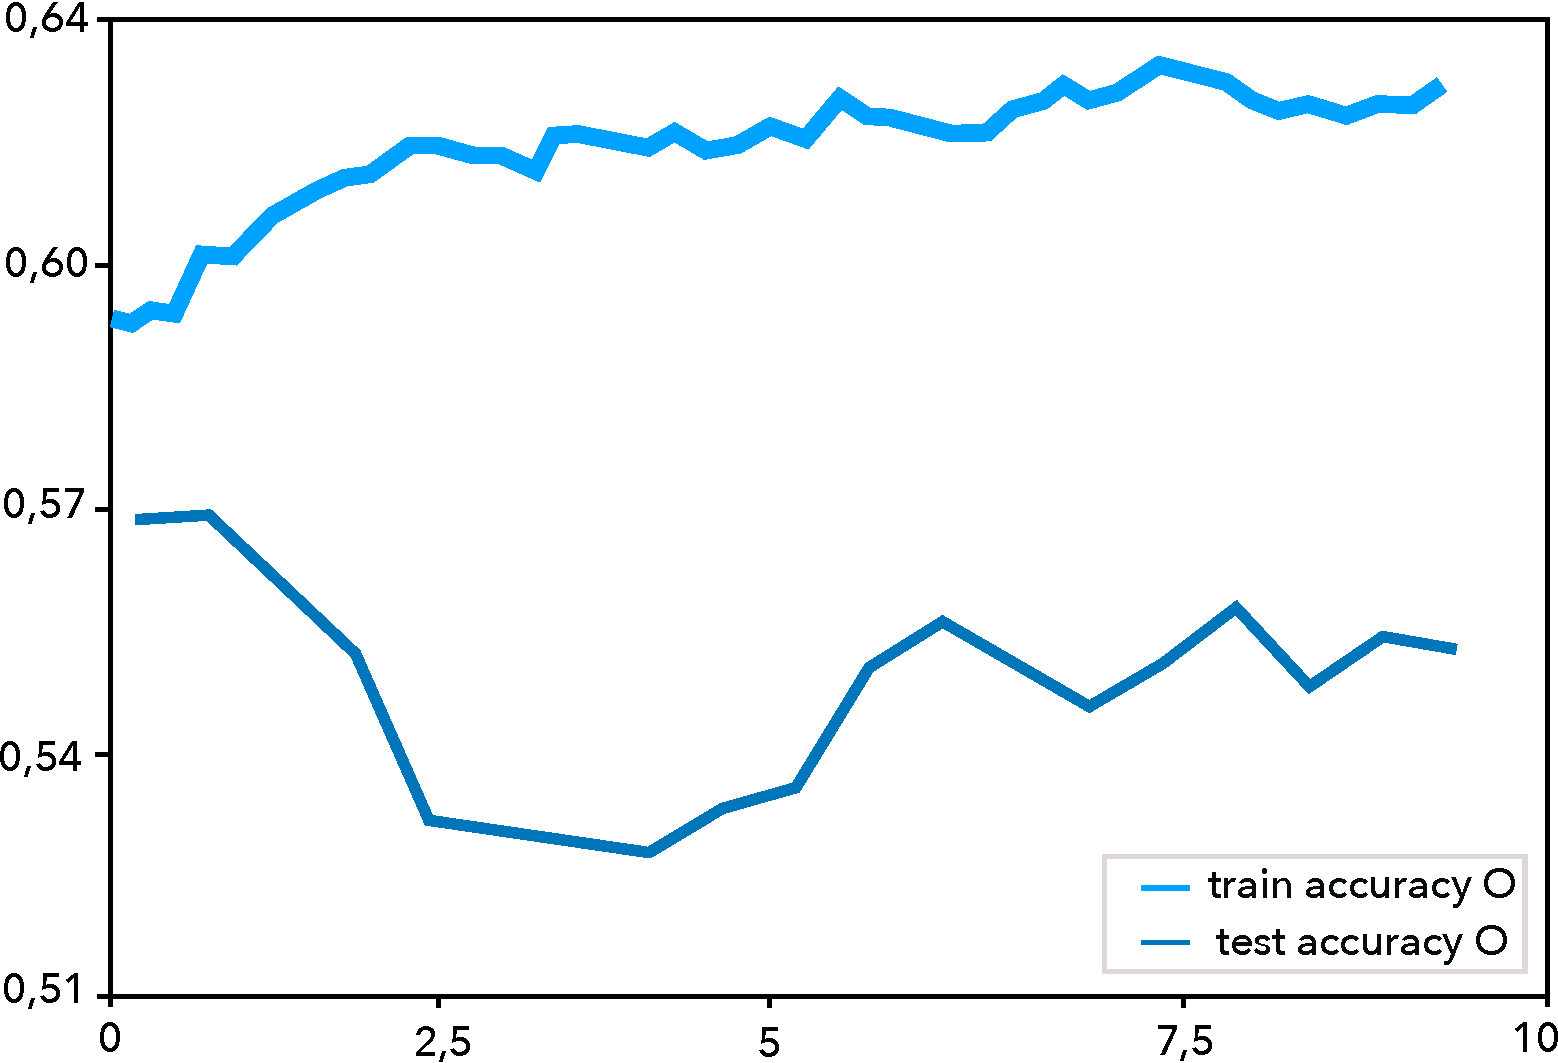
\includegraphics[width=.8\textwidth]{images/binary/plotO}
		\end{minipage}}
	\caption{Analisi della caratteristica Openness del ``Modello 13''}
	\label{fig:binO}
\end{figure}

\begin{figure}[H]
	\centering
	\subfloat[][\emph{Visualizzazione matrice di confusione}\label{subfig:confC}]
	{\begin{minipage}[c][0.7\width]{0.45\textwidth}
			\centering
			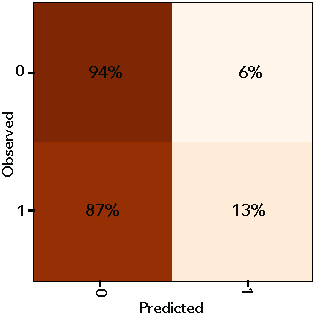
\includegraphics[width=.6\textwidth]{images/binary/accC}
		\end{minipage}} 
	\hspace{10mm}
	\subfloat[][\emph{Visualizzazione accuratezza su train e test}\label{subfig:accC}]
	{\begin{minipage}[c][0.7\width]{0.45\textwidth}
			\centering
			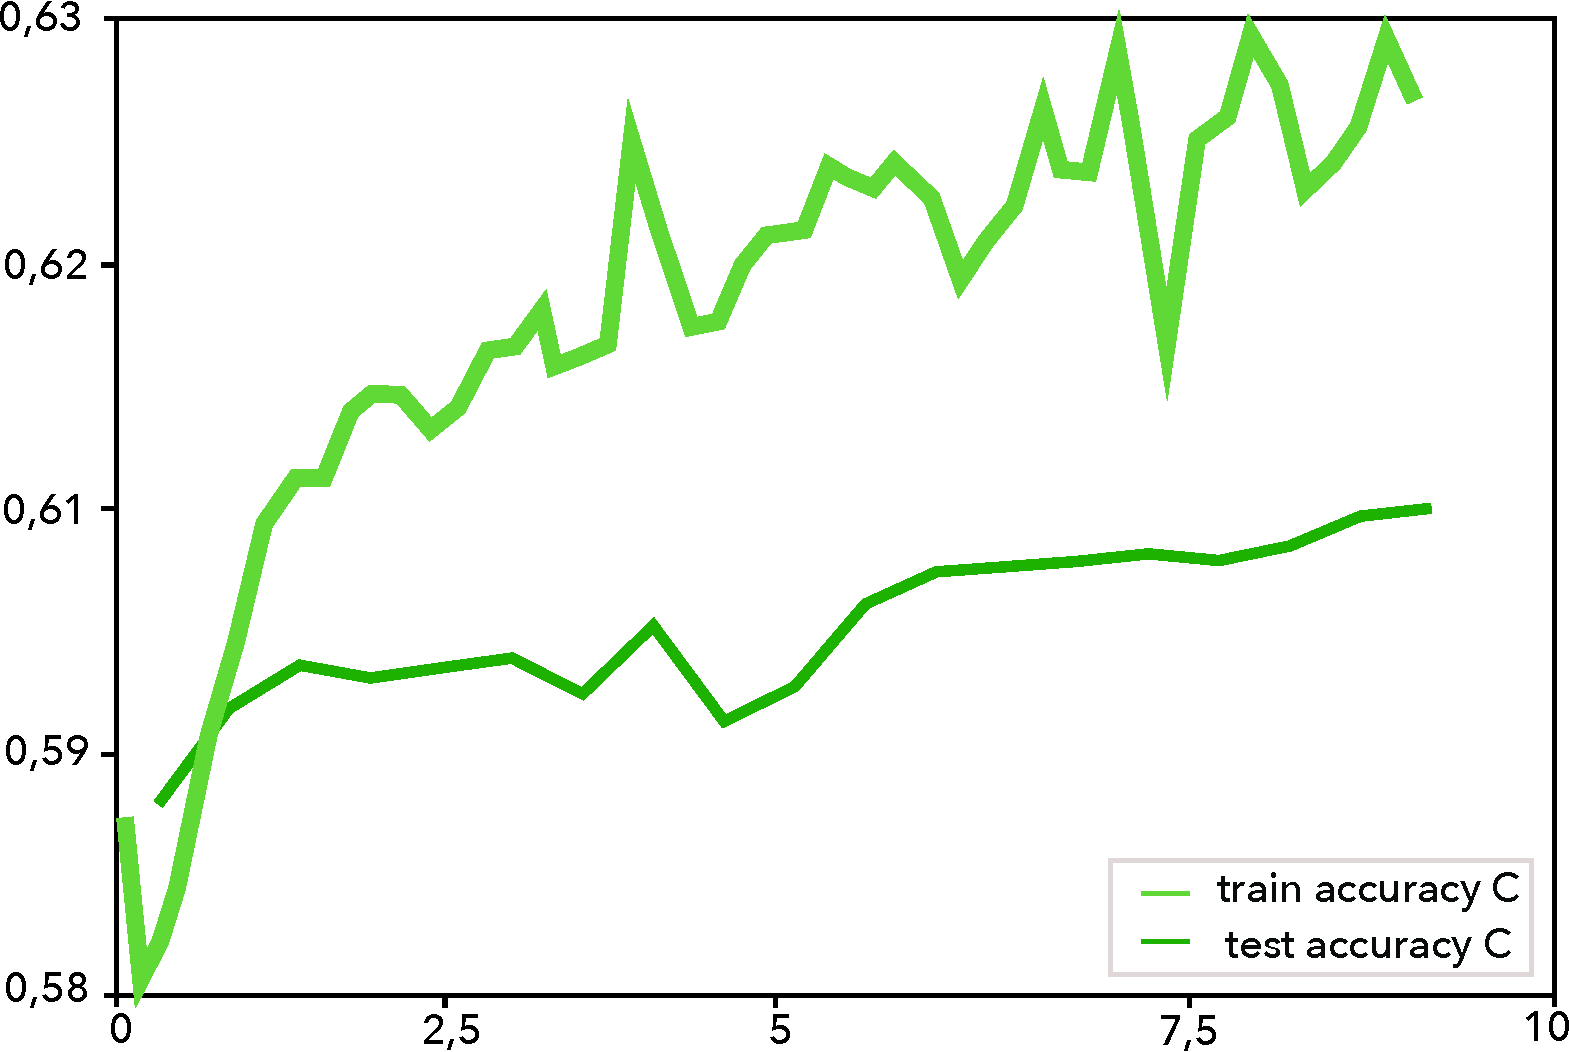
\includegraphics[width=.8\textwidth]{images/binary/plotC}
		\end{minipage}}
	\caption{Analisi della caratteristica Conscientiousness del ``Modello 13''}
	\label{fig:binC}
\end{figure}

\begin{figure}[H]
	\centering
	\subfloat[][\emph{Visualizzazione matrice di confusione}\label{subfig:confE}]
	{\begin{minipage}[c][0.7\width]{0.45\textwidth}
			\centering
			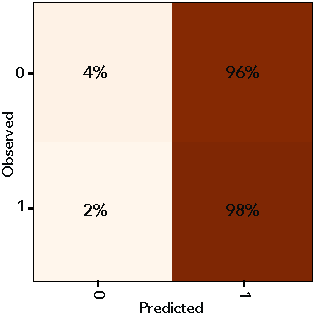
\includegraphics[width=.6\textwidth]{images/binary/accE}
		\end{minipage}} 
	\hspace{10mm}
	\subfloat[][\emph{Visualizzazione accuratezza su train e test}\label{subfig:accE}]
	{\begin{minipage}[c][0.7\width]{0.45\textwidth}
			\centering
			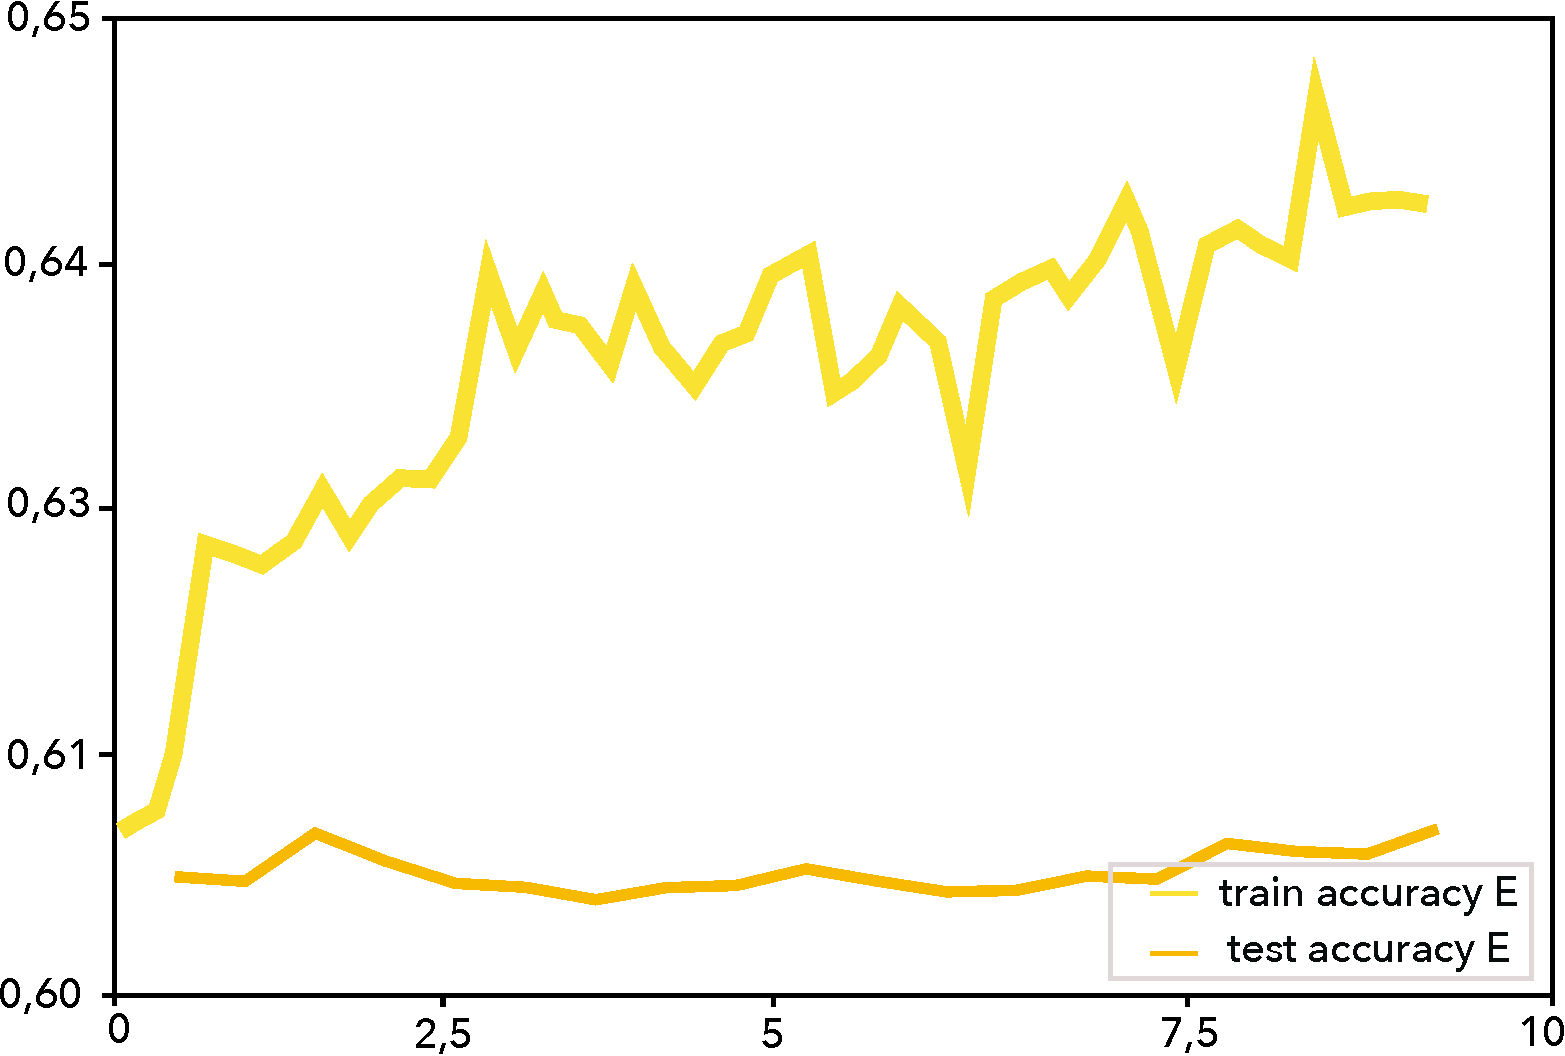
\includegraphics[width=.8\textwidth]{images/binary/plotE}
		\end{minipage}}
	\caption{Analisi della caratteristica Extraversion del ``Modello 13''}
	\label{fig:binE}
\end{figure}

\begin{figure}[H]
	\centering
	\subfloat[][\emph{Visualizzazione matrice di confusione}\label{subfig:confA}]
	{\begin{minipage}[c][0.7\width]{0.45\textwidth}
			\centering
			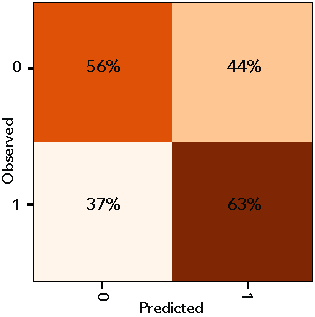
\includegraphics[width=.6\textwidth]{images/binary/accA}
		\end{minipage}} 
	\hspace{10mm}
	\subfloat[][\emph{Visualizzazione accuratezza su train e test}\label{subfig:accA}]
	{\begin{minipage}[c][0.7\width]{0.45\textwidth}
			\centering
			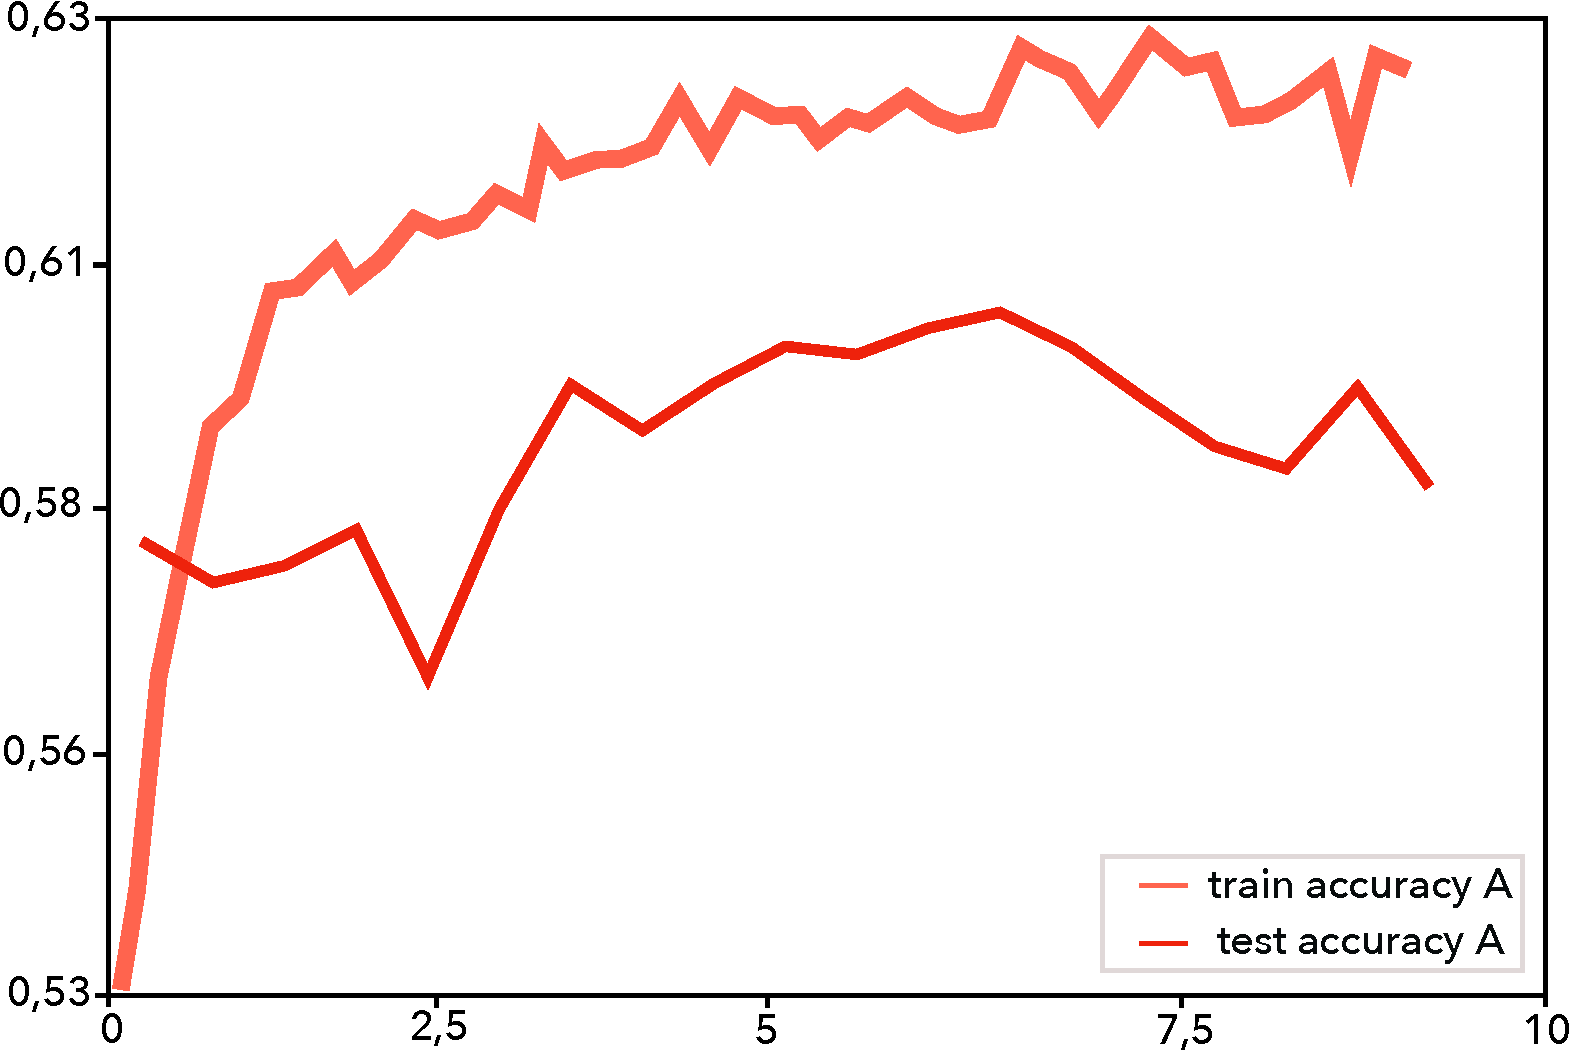
\includegraphics[width=.8\textwidth]{images/binary/plotA}
		\end{minipage}}
	\caption{Analisi della caratteristica Agreeableness del ``Modello 13''}
	\label{fig:binA}
\end{figure}

\begin{figure}[H]
	\centering
	\subfloat[][\emph{Visualizzazione matrice di confusione}\label{subfig:confN}]
	{\begin{minipage}[c][0.7\width]{0.45\textwidth}
			\centering
			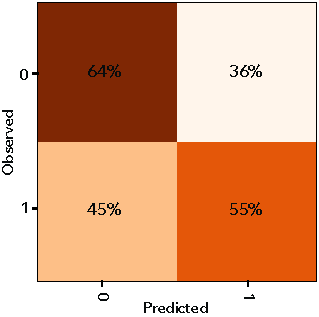
\includegraphics[width=.6\textwidth]{images/binary/accN}
		\end{minipage}} 
	\hspace{10mm}
	\subfloat[][\emph{Visualizzazione accuratezza su train e test}\label{subfig:accN}]
	{\begin{minipage}[c][0.7\width]{0.45\textwidth}
			\centering
			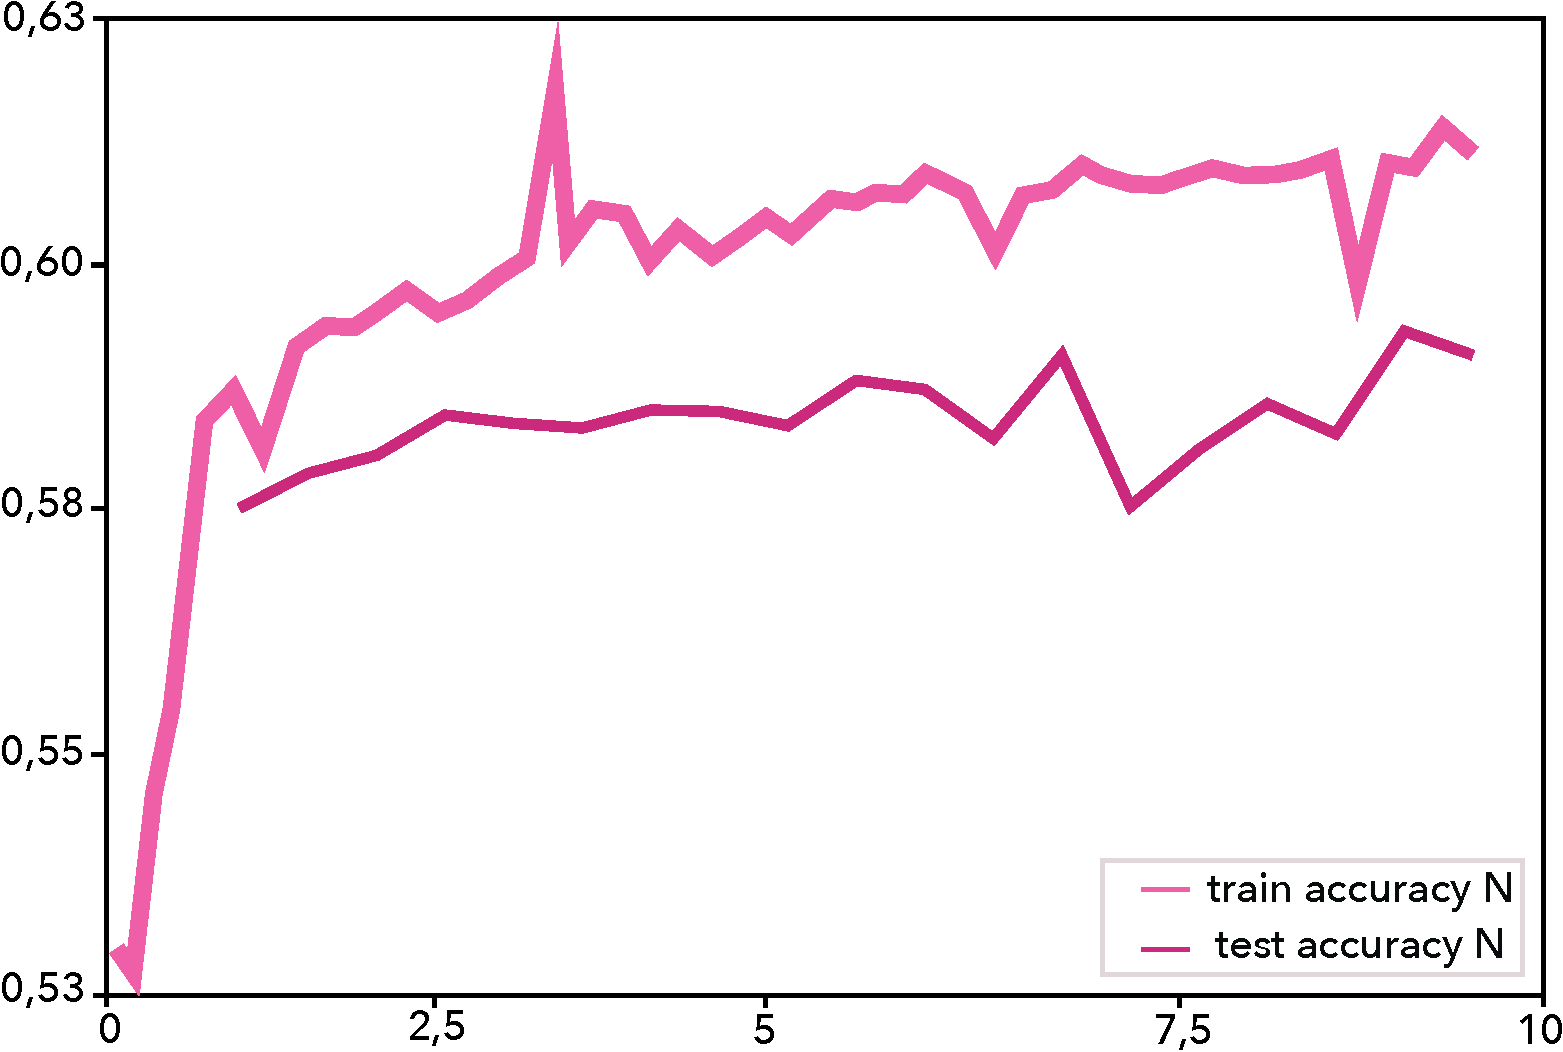
\includegraphics[width=.8\textwidth]{images/binary/plotN}
		\end{minipage}}
	\caption{Analisi della caratteristica Neuroticism del ``Modello 13''}
	\label{fig:binN}
\end{figure}

